\chapter{Validation of Motivation Surveys}
\label{appendix:validation-motivation-surveys}

This appendix details the validation process on the motivation surveys employed in the empirical studies of this PhD dissertation. These instruments are the Intrinsic Motivation Inventory (IMI) and the Instructional Materials Motivation Survey (IMMS). Both instruments have been adapted and translated from their original English versions into Portuguese by the thesis author to measure the students' motivation regarding to their participation in CL sessions. Thus, the validation and reliability analysis presented here ensure that the translated items are psychometrically sound. The procedure for the validation and reliability tests is presented in \autoref{sec:validation-motivation-surveys-process}, and the results of this procedure is detailed in \autoref{sec:validation-motivation-surveys-results}.

\section{Validation Procedure}
\label{sec:validation-motivation-surveys-process}

\subsection{Participants}

The collected data to conduct the validation and reliability tests of the motivation surveys come from 103 undergraduate Brazilian students who were enrolled in the first year of bachelor degree programs in computer science and computer engineering at the University of São Paulo. 37 of these participants were students signed up on the course \aspas{Introduction to Computer Science} for the second semester of 2016 (September-December), and 66 of them were students signed up on the course for the first semester of 2017 (March-July). These participants were in the age range from 18 to 25 years old, sharing similar social-economy status and culture.

\subsection{Instruments}

\subsubsection*{Intrinsic Motivation Inventory (IMI)}

The IMI is a psychometric instrument in which the Self-Determinant Theory (SDT) has been used as theoretical fundament to define seven scales (Interest/Enjoyment, Perceived Choice, Perceived Competence, Pressure/Tension, Effort/Importance, Value/Usefulness, and Relatedness) to measure the intrinsic motivation of participants towards a target activity \cite{MonteiroMataPeixotoMonteiroMataPeixoto2015, RyanDeci2000}. According to the authors of this instrument, no all the scales are needed to measure the intrinsic motivation, the scales can be selected according to the situation, removing those that are redundant and those that are not in accordance to the situation. In the adapted Portuguese IMI, four scales have been selected by the thesis author to measure the intrinsic motivation of Brazilian students towards their participation in CL sessions. These sub-scales are: the Interest/Enjoyment, Perceived Choice, Pressure/Tension, and Effort/Importance.

The Interest/Enjoyment is the self-report direct measure of intrinsic motivation whereby the items related to this scale has been included in the adapted Portuguese IMI. The Perceived Choice and Perceived Competence are both scales defined as positive predictors of the intrinsic motivation, so that the items related to the Perceived Competence had been removed from the instrument, and items related to the Perceived Choice have been selected as the only positive predictor. Furthermore, the scale of the perceived choice has been selected to measure the intrinsic motivation because the thesis author hypothesizes that the scripted collaboration increases the feeling of obligation in the participants. Items related to the Pressure/Tension have been included in the adapted Portuguese IMI as the negative predictor of intrinsic motivation. Items related to the scale of Effort/Importance has been included in the adapted Portuguese IMI to measure the internalization of motivation. Items related to the scale of Relatedness have not been included in the adapted Portuguese IMI because this scale intends to measure the feeling to be connected to others participants in target activity where the goal of activity is obtain interpersonal relationships.

Three questionnaires of the adapted Portuguese IMI had been used to collect the students' motivation data over the empirical studies. These questionnaires in the paper-based version (Annex \ref{annex:IMI-first-study}) and web-based version (Annex \ref{annex:IMI-pilot-study} and Annex \ref{annex:IMI-IMMS-third-study}) comprised 24 items, with all the items scored on a 7-point Likert scale using the ranging from 1 (\emph{not at all}) to 7 (\emph{very true}).

\subsubsection*{Instructional Materials Motivation Survey (IMMS)}

The IMMS is the psychometric instrument developed by \citeonline{Keller2009} to assess the students' motivational attitude towards instructional materials or courses. This instrument has been developed in correspondence with the ACRS model, thereby the scales of of Attention, Relevance, Confidence and Satisfaction (ARCS) are used to measure the reaction of students to instructional materials or course, and this reaction is then considered a self-report measure to the students' motivational attitude.

Instead to use the 36 items defined in the original version of IMMS, the adapted Portuguese IMMS has been defined using only 25 item. 11-items related to the scale of \emph{C: Confidence} have been removed from the instrument, because the scales of \emph{C: Confidence} and \emph{PC: Perceived Choice} measure the self-regulation of an individual. Removing the scale of Confidence in the adapted Portuguese IMMS avoid an overloading of work for the participants when they were requested to answered the questionnaires. Furthermore, the author of the original version of IMMS indicates that each one of the four scales defined in the IMMS could be used and scored independently \cite{Keller2009}. Thus, in the adapted Portuguese IMMS, the students' motivational attitude towards the CL sessions had been measured as the \emph{LM: Level of Motivation}, a measure that consists in the scales of \emph{A: Attention}, \emph{R: Relevance}, and \emph{S: Satisfaction}. 

Two questionnaires of the adapted Portuguese IMMS had been used to collect the students' motivation data over the empirical studies. These questionnaires in the paper-based version (Annex \ref{annex:IMMS-second-study}) and web-based version (Annex \ref{annex:IMI-IMMS-third-study} had been scored on a 7-point Likert scale using the ranging from 1 (\emph{not at all}) to 7 (\emph{very true}).

\subsection{Data Collection Procedure}

Web-based questionnaires of the motivation surveys were used to collect the responses through the Moodle platform during the pilot and third empirical studies, and paper-based questionnaires of these surveys were used at the classroom to collect the responses during the first empirical study. During the pilot study, 32 responses to the adapted Portuguese IMI were collected from the 37 computer science students by means of a web-based questionnaire (detailed in Annex \ref{annex:IMI-pilot-study}). During the first empirical study, 62 responses to the adapted Portuguese IMI were collected from the 66 computer engineering students by means of a paper-based questionnaire (detailed in Annex \ref{annex:IMI-first-study}). During the second empirical study, 58 responses to the adapted Portuguese IMMS were collected from the 66 computer engineering students by means a paper-based questionnaire (detailed in Annex \ref{annex:IMMS-second-study}). During the third empirical study, 55 responses to the adapted Portuguese IMI and the adapted Portuguese IMMS were collected by means of a web-based questionnaire (detailed in Annex \ref{annex:IMI-IMMS-third-study}).

\subsection{Data Analysis}

Although the common statistical advice to perform the validation of surveys indicates a minimum sample size of 300 observations \cite{Kline1986}, recent simulations demonstrated that the validation process is possible with small samples under certain circumstances \cite{GuadagnoliVelicer1988, RouquetteFalissard2011, Yurdugul2008}. According to these studies, to conduct the validation of surveys and the reliability tests of them with small samples, the items must sufficiently correspond to the scale for which they are intended, and the Cronbach’s alpha coefficient ($\alpha$) must be stable in this small sample. Thus, the correspondence of items and scales had been validated by a factorial analysis using \emph{varimax} rotation, and the items with a component loading less than 0.40 and those with a cross-loading value less than 0.20 had been removed from the instrument. The stability of Cronbach’s alpha ($\alpha$) had been evaluated using the cut-off values defined by \citeonline{Yurdugul2008}. According to these cut-off values, if the sample size is between 30 and 50 observations, and the level of the first eigenvalue is less than 6, the Cronbach’s alpha ($\alpha$) is not stable; if the sample size is between 50 and 100, and the level of the first eigenvalue is between 3 and 6, the Cronbach’s alpha ($\alpha$) is stable, but an informed decision must be conducted by reviewing the literature and/or consulting with specialists to confirm the number of scales; and if the sample is between 100 and 300 observation and the level of the first eigenvalue is between 1 to 3, the Cronbach’s alpha ($\alpha$) is stable but a informed decision should be conducted to define the number of scales.

After to verify the correspondence of the items with the scales and to ensure the stability of Cronbach’s alpha ($\alpha$), the structure of the items in the motivation surveys had been evaluated with a Confirmatory Factor Analysis (CFA) by testing three different models: multidimensional, second order and bi-factor models. To select the model that best fits for the collected data, the CFA had been carried out using the diagonally weighted least squares (WLSMV) estimator. The WLSMV estimator is a estimator specifically designed for small samples with ordinal data (such the 7-point Likert scale used in the IMI and IMMS), and it makes no distributional assumptions about the observed variables \cite{Brown2014,Li2016,RhemtullaBrosseau-LiardSavalei2012}. The result of CFA is a set of goodness fit indices used to select the model that best fits for the collected data. These indices were: Chi-square (${\chi}^2$), Adjusted Goodness of Fit Index (AGFI), the Tucker-Lewis Index (TLI), the Comparative Fit Index (CFI) and the Root Mean Square Error of Approximation (RMSEA). As the ${\chi}^2$ is highly sensitive to the sample size \cite{HuBentler1999}, this indicator was only be used in the case that the others indicators do not significantly differ in relation with the others models. In this case, the model that best fits with the collected data is the model with smaller Chi-square (${\chi}^2$). Values between 0.90 to 0.95 were considered acceptable thresholds for the indices of AGFI, TLI and CFI; and values higher than 0.96 were considered good fit. The RMSEA obtained by the CFA had been a scaled value of the RMSEA, so that it was considered acceptable when the value was 0.10s and good when the value was less than 0.10. After to select the model that best fits for the collected data, separate reliability tests had been conducted in the global sample and the samples obtained in each empirical study to evaluate the consistency of the motivation surveys. In these tests, values in the Cronbach’s alpha ($\alpha$) greater than 0.70 were considered as acceptable, and values above 0.80 were considered as highly reliable.

The CFA and reliability tests had been carried out in R software version 3.4.3 \cite{RCoreTeam2017} using the lavaan package version 0.5 \cite{Rosseel2012} for the CFA, and the psych package version 1.7.8 \cite{Revelle2017} for the reliability tests. The R scripts for the validation of the adapted Portuguese IMI and the adapted Portuguese IMMS are available, with the data files, at the URL: \url{https://geiser.github.io/phd-thesis-evaluation/} 

\section{Results}
\label{sec:validation-motivation-surveys-results}

Prior to the data analysis detailed above, the outliers identified as careless responses had been removed from the data, and the outliers identified as extreme values had been treated using the winsorization method. The detection and treatment of these outliers is detailed in \autoref{sec:outliers-motivation}. After to remove the careless responses, the global sample size employed to obtain the results presented here were 141 observations and 110 observations to validate the adapted Portuguese IMI and IMMS, respectively. To validate the Portuguese adapted IMI, the data consisted in 30 observations from the pilot study, 60 observations from the first empirical study, and 51 observations from the third empirical study. To validate the Portuguese adapted IMMS, the data consisted in 58 observations from the empirical study and 52 observations from the third empirical study.

\subsection{Factorial Structure of the Adapted Portuguese IMI}

\autoref{fig:imi-models-cfa} shows the multidimensional, second-order factor and bi-factor models that had been tested in the CFA to validate the factorial structure of the adapted Portuguese IMI. The construction of these models had been conducted according to the criteria defined in the validation procedure by removing items that had loaded with a value less than 0.4, and also, by removing items that had cross-loading less than 0.2. This construction ensures that the items correspond to the scale for which they are intended, and that the Cronbach’s $\alpha$ is stable.

\begin{figure}[htb!]
 \caption{Models tested in the CFA to validate the factorial structure of the adapted Portuguese IMI}
 \label{fig:imi-models-cfa}
 \centering
 \begin{tabular}{ccc}
 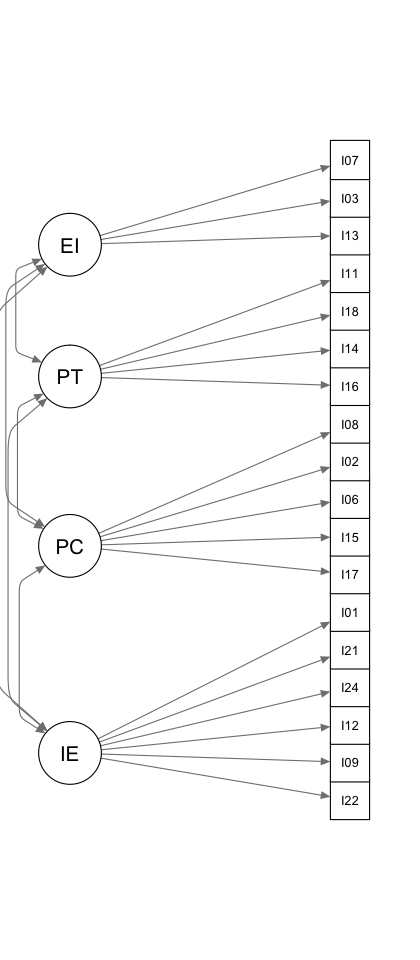
\includegraphics[width=0.25\textwidth]{images/appendix/imi-multidimensional-model.png} &
 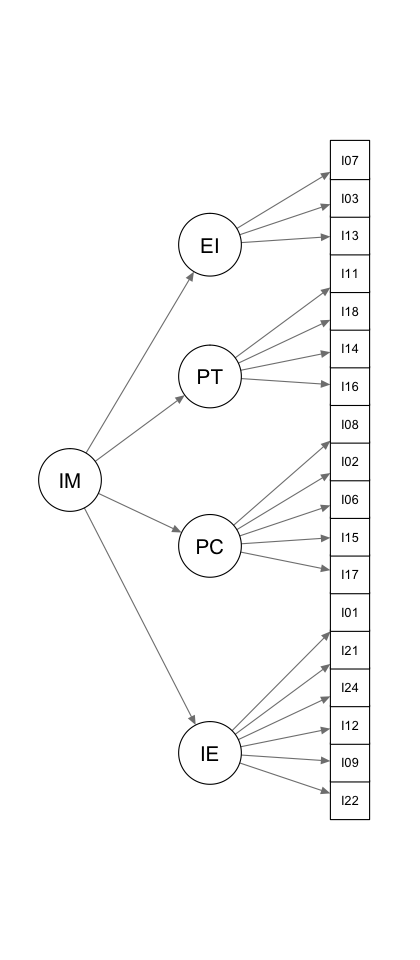
\includegraphics[width=0.25\textwidth]{images/appendix/imi-second-order-factor-model} &
 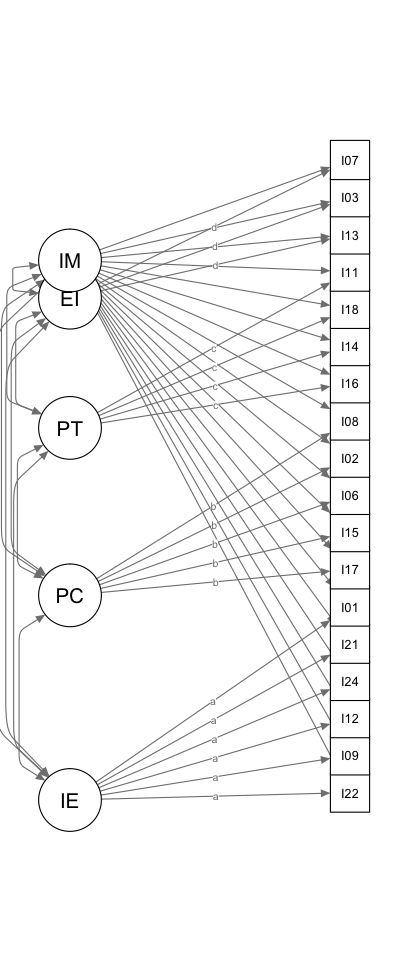
\includegraphics[width=0.25\textwidth]{images/appendix/imi-bi-factor-model.png} \\
 {\scriptsize multidimensional model} & {\scriptsize second-order factor model} & {\scriptsize bi-factor model} \\
 \end{tabular}
 \fautor
\end{figure}

As result of the construction of these models, the Item 19 - \aspas{\emph{Achei que a atividade seria chata}} as translated version of \aspas{I thought this was a boring activity} - was removed from the factorial structure because it loads in  the scale of \emph{PC: Perceived Choice} for which it does not have concordance. The Item 04 - \aspas{\emph{Para mim foi importante realizar bem a atividade}} as a translated version of \aspas{It was important to me to do well at this task} - was also removed from the factorial structure because it does not load in the scale of \emph{EI: Effort/Importance} for which it was intended, and because it loads in the scale of \emph{IE: Interest/Enjoyment} where it lacks of concordance. Instead to load in the scale of \emph{PT: Pressure/Tension}, the Item01 - \aspas{\emph{Foi muito descontraido realizar a ativide}} as the translated version of \aspas{I was very relaxed in doing the activity} - loaded in the the scale of \emph{IE: Interest/Enjoyment} because the word \aspas{\emph{descontraido}} was understood by the participants in the sense of enjoyment rather than the pressure. Thus, the Item 01 has been used as an item to measure the Interest/Enjoyment rather than to measure the Pressure/Tension.

\autoref{tab:imi-goodness-fit} shows the goodness fit statistics for the models tested in the validation of the adapted Portuguese IMI. The results presented in this table indicate that all the models have adequate goodness fit indices for all the samples (the global sample, and the data collected over the pilot, first and third empirical studies). The bi-factor model had not converged for the data collected over the third empirical study, and the second-order factor model had partially converged for those data. According to this results, the model that best fits the global sample is the second-order factor model with ${\chi}^2 = 63.27$ that outperforms the multidimensional model (${\chi}^2 = 80.08$) and the bi-factor model (${\chi}^2 = 86.28$). The AGFI index for the multidimensional model and the second-order factor model are better that the AGFI index for the bi-factor model. In relation to the TLI and CFI indices, the the second-order factor model with $TLI = 0.90$ and $CFI = 0.82$ outperforms the multidimensional model ($TLI = 0.89$ and $CFI = 0.76$), and the bi-factor model ($TLI = 0.84$ and $CFI = 0.72$). The RMSEA of all models are acceptable for a robust estimation with a good value for the lower limit in the confidence interval.

%latex.default(round(fitMeasures_df, 2), caption = paste("Goodness of fit statistics",     in_title), size = "scriptsize", longtable = T, ctable = F,     landscape = F, rowlabel = "", where = "!htbp", file = filename,     append = T)%
\setlongtables{\footnotesize
\begin{longtable}{lrrrrrrrr}
\caption{Goodness of fit statistics in the validation of the adapted Portuguese IMI}
\tabularnewline
\hline\hline
\multicolumn{1}{l}{}&\multicolumn{1}{c}{df}&\multicolumn{1}{c}{${\chi}^2$}&\multicolumn{1}{c}{AGFI}&\multicolumn{1}{c}{TLI}&\multicolumn{1}{c}{CFI}&\multicolumn{1}{c}{RMSEA}&\multicolumn{1}{c}{CI.lwr}&\multicolumn{1}{c}{CI.upr}\tabularnewline
\hline
\endfirsthead\caption[]{\em (continued)} \tabularnewline
\hline
\multicolumn{1}{l}{}&\multicolumn{1}{c}{df}&\multicolumn{1}{c}{${\chi}^2$}&\multicolumn{1}{c}{AGFI}&\multicolumn{1}{c}{TLI}&\multicolumn{1}{c}{CFI}&\multicolumn{1}{c}{RMSEA}&\multicolumn{1}{c}{CI.lwr}&\multicolumn{1}{c}{CI.upr}\tabularnewline
\hline
\endhead
\hline
\multicolumn{9}{r}{\tiny df: degree of freedom; AGFI: Adjusted Goodness of Fit Index; CFI: Comparative Fit Index; TLI: Tucker-Lewis Index;}\tabularnewline \multicolumn{9}{r}{\tiny RMSEA: Root Mean Square Error of Approximation}
\endfoot
\label{tab:imi-goodness-fit}
Global sample: Multidimensional model&$ 26.59$&$80.08$&$0.99$&$0.89$&$0.76$&$0.12$&$0.10$&$0.14$\tabularnewline
Global sample: Second-order factor model&$ 23.35$&$63.27$&$0.99$&$0.90$&$0.82$&$0.11$&$0.09$&$0.13$\tabularnewline
Global sample: Bi-factor model&$ 22.70$&$86.28$&$0.98$&$0.84$&$0.72$&$0.14$&$0.12$&$0.16$\tabularnewline \hline
Pilot study: Multidimensional model&$  8.25$&$14.30$&$0.96$&$0.83$&$0.86$&$0.16$&$0.11$&$0.21$\tabularnewline
Pilot study: Second-order factor model&$  7.88$&$14.06$&$0.96$&$0.82$&$0.85$&$0.16$&$0.11$&$0.21$\tabularnewline
Pilot study: Bi-factor model&$  9.90$&$18.39$&$0.97$&$0.80$&$0.80$&$0.17$&$0.11$&$0.23$\tabularnewline \hline
First study: Multidimensional model&$ 18.93$&$25.80$&$0.99$&$0.92$&$0.87$&$0.08$&$0.02$&$0.12$\tabularnewline
First study: Second-order factor model&$ 17.92$&$26.26$&$0.98$&$0.90$&$0.84$&$0.09$&$0.05$&$0.13$\tabularnewline
First study: Bi-factor model&$ 17.83$&$34.68$&$0.98$&$0.80$&$0.68$&$0.13$&$0.09$&$0.16$\tabularnewline \hline
Third study: Multidimensional model&$ 16.43$&$30.22$&$0.98$&$0.85$&$0.76$&$0.13$&$0.09$&$0.17$\tabularnewline
Third study: Second-order factor model&$131.00$&$$&$0.97$&$$&$$&$$&$0.00$&$0.00$\tabularnewline
Third study: Bi-factor model&$$&$$&$$&$$&$$&$$&$$&$$\tabularnewline
\hline
\end{longtable}
}

In relation to the data collected in each empirical study, the goodness of fit statistics in the validation of the adapted Portuguese IMI (shown in \autoref{tab:imi-goodness-fit}) have slight differences. For the data collected over the pilot study, the second-order factor model with ${\chi}^2=14.06$ fits better than the multidimensional model and the bi-factor model but the difference is not significant. For the data collected over the first empirical study, the multidimensional model with ${\chi}^2=25.80$ outperforms the bi-factor model and the multidimensional model. For the data collected over the third empirical study, the multidimensional model with ${\chi}^2=30.22$ is the only model that had converged in the simulation.

%latex.default(fa_summary_df, caption = paste("Summary of exploratory and confirmatory factor analysis for the",     in_title), size = "small", longtable = T, ctable = F, landscape = F,     rowlabel = "", where = "!htbp", file = filename, append = T)%
\setlongtables{\footnotesize
\begin{longtable}{lrrrr}\caption{Summary of the factor analysis for the adapted Portuguese IMI} \tabularnewline
\hline\hline
\multicolumn{1}{l}{}&\multicolumn{1}{c}{MR1}&\multicolumn{1}{c}{MR3}&\multicolumn{1}{c}{MR2}&\multicolumn{1}{c}{MR4}\tabularnewline
\hline
\endfirsthead\caption[]{\em (continued)} \tabularnewline
\hline
\multicolumn{1}{l}{}&\multicolumn{1}{c}{MR1}&\multicolumn{1}{c}{MR3}&\multicolumn{1}{c}{MR2}&\multicolumn{1}{c}{MR4}\tabularnewline
\hline
\endhead
\hline
\multicolumn{5}{r}{\tiny CFI: 0.822; TLI: 0.904; df: 23.354; ${\chi}^2$: 63.271; RMSEA: 0.11 [0.09, 0.132];}
\endfoot
\label{tab:imi-factor-loading}
\emph{IE: Interest/Enjoyment} & & & & \tabularnewline
Item22: \emph{Achei a atividade muito agradável} &$ 0.837$&$-0.237$&$-0.111$&$-0.073$\tabularnewline
Item09: \emph{Gostei muito de fazer a atividade} &$ 0.828$&$-0.256$&$-0.168$&$-0.106$\tabularnewline
Item12: \emph{A atividade foi divertida} &$ 0.827$&$-0.218$&$-0.157$&$-0.092$\tabularnewline
Item24: \emph{Enquanto estava fazendo a atividade, refleti ...} &$ 0.787$&$ 0.024$&$-0.060$&$-0.188$\tabularnewline
Item21: \emph{Descreveria a atividade como muito interessante} &$ 0.772$&$-0.210$&$ 0.052$&$-0.093$\tabularnewline
Item01: \emph{Foi muito descontraído realizar a atividade} &$ 0.691$&$-0.234$&$-0.216$&$-0.012$\tabularnewline \hline
\emph{PC: Perceived Choice} & & & & \tabularnewline
Item17: \emph{Fiz a atividade porque eu não tinha outra escolha} &$-0.168$&$ 0.802$&$ 0.246$&$ 0.184$\tabularnewline
Item15: \emph{Fiz a atividade porque eu tinha que fazer} &$-0.132$&$ 0.721$&$ 0.070$&$ 0.053$\tabularnewline
Item06: \emph{Realmente não tive escolha para realizar ...} &$-0.108$&$ 0.748$&$ 0.133$&$ 0.012$\tabularnewline
Item02: \emph{Senti como se eu tivesse sido obrigado ...} &$-0.270$&$ 0.707$&$ 0.167$&$-0.020$\tabularnewline
Item08: \emph{Senti que não fiz a atividade por vontade ...} &$-0.360$&$ 0.651$&$ 0.214$&$ 0.240$\tabularnewline \hline
\emph{PT: Pressure/Tension} & & & & \tabularnewline
Item16: \emph{Eu me senti ansioso enquanto trabalhava ...} &$ 0.040$&$ 0.197$&$ 0.839$&$-0.056$\tabularnewline
Item14: \emph{Eu me senti muito tenso ao realizar a atividade} &$-0.121$&$ 0.245$&$ 0.788$&$ 0.110$\tabularnewline
Item18: \emph{Seti-me pressionado enquanto fazia a atividade} &$-0.157$&$ 0.386$&$ 0.739$&$ 0.089$\tabularnewline
Item11: \emph{Não me senti nervoso ao realizar a atividade} &$ 0.365$&$ 0.043$&$-0.636$&$ 0.037$\tabularnewline \hline
\emph{EI: Effort/Importance} & & & & \tabularnewline
Item13: \emph{Não me esforcei muito para realizar bem atividade} &$-0.030$&$ 0.184$&$ 0.185$&$ 0.708$\tabularnewline
Item03: \emph{Me esforcei muito na realização da atividade} &$ 0.276$&$ 0.041$&$ 0.194$&$-0.650$\tabularnewline
Item07: \emph{Não coloquei muita energia (esforço) na atividade} &$-0.062$&$ 0.076$&$ 0.031$&$ 0.691$\tabularnewline \hline
SS loadings&$ 4.280$&$ 3.206$&$ 2.624$&$ 1.589$\tabularnewline
Cumulative Var&$ 0.238$&$ 0.416$&$ 0.562$&$ 0.650$\tabularnewline
Proportion Explained&$ 0.366$&$ 0.274$&$ 0.224$&$ 0.136$\tabularnewline
\hline
\end{longtable}}

\autoref{tab:imi-factor-loading} shows the summary of the factor analysis conducted with the global sample for the adapted Portuguese IMI. The factor loadings, eigenvalues, cumulative variance and proportion explained by the items indicates the emergence of four factors: Interest/Enjoyment (F1), Perceived Choice (F2), Pressure/Tension (F3), and Effort/Importance (F4). The items in the first factor (F1: Interest/Enjoyment) have strong primary loadings with values greater than 0.6, and the majority of proportion (36\%) is explained  by the first factor. These results are similars to the findings obtained in previous validation of the IMI conducted by \citeonline{McAuleyDuncanTammen1989, MarklandHardy1997, MonteiroMataPeixotoMonteiroMataPeixoto2015}. According to the cut-off value defined by \citeonline{Yurdugul2008}, the first eigenvalue has a level of $4.2$ indicating stability in the Cronbach’s $\alpha$ for a sample size ($N=141$) between 100 to 300 observation.

\subsection{Reliability Tests of the Adapted Portuguese IMI}

The overall and internal consistency of the adapted Portuguese IMI had been evaluated by reliability tests in the global sample, and in the data collected over each empirical study (the pilot study, and the first and third studies). \autoref{tab:reliability-IMI} shows the results of the reliability tests in which the Cronbach's alpha ($\alpha$) for the Intrinsic Motivation have good overall consistency for the global sample and the data collected in each empirical study with values greater than 0.80. The Cronbach's alpha ($\alpha$) in the scales of \emph{IE: Interest/Enjoyment}, \emph{PC: Perceived Choice}, \emph{PT: Pressure/Tension} indicate good consistency and high reliability for all the samples with values greater than $0.70$ and $0.80$. The Cronbach's alpha ($\alpha$) in the scale of \emph{EI: Effort/Importance} indicate an acceptable consistency for the global sample and the data collected over the third empirical study. Although the Cronbach's alpha ($\alpha$) in the scale of \emph{EI: Effort/Importance} have values less than 0.70 for the data collected over the pilot and first studies, these values ($\alpha_{pilot} = 0.699$ and $\alpha_{third} = 0.692$) are consider acceptable because they are close to $0.70$.

Separate reliability tests had also been conducted in the adapted Portuguese IMI for the collected data in each empirical study and by dividing this data into: responses from students who participated in non-gamified CL sessions (\emph{non-gamified}), responses from students who participated in ontology-based CL sessions (\emph{ont-gamified}), and responses from students who participated in CL sessions that had been gamified without using ontologies (\emph{w/o-gamified}). \autoref{tab:reliability-IMI-samples} shows the results of these reliability tests. For the data collected over the pilot study where the groups of responses had been divided into ont-gamified CL sessions and non-gamified CL sessions, the results of reliability tests indicate, in the majority of scales and groups, highly consistent with good (Cronbach's $\alpha$ in $0.80$s) and excellent (Cronbach's $\alpha$ in $0.90$s) internal consistency. The Cronbach's $\alpha$ indicates only questionable internal consistency for the \aspas{\emph{ont-gamified}} group in the scale of \emph{PT: Pressure/Tension} with a Cronbach's alpha $\alpha = 0.608$. In the scale of \emph{EI: Effort/Importance}, the reliability test for the \aspas{\emph{non-gamified}} group indicates a Cronbach's $\alpha = 0.690$ that is a value close to the threshold of 0.70 by which its internal consistency is consider acceptable.

For the data collected over the first empirical study where the groups of responses had been divided into ont-gamified CL sessions and w/o-gamified CL sessions, the results of reliability tests indicates good and excellent internal consistency in all the scales and groups, the only exception occurs for the \aspas{\emph{ont-gamified}} group in the scale of \emph{EI: Effort/Importance} that indicates a questionable consistency with a Cronbach's $\alpha = 0.632$. For the data collected over the third empirical study where the groups of responses had been divided into ont-gamified CL sessions and w/o-gamified CL sessions, the results of reliability tests shows highly internal reliability in all the scales and groups. Only, the result in the group \aspas{\emph{ont-gamified}} for the scale of \emph{EI: Effort/Importance} indicates a poor internal consistency with a Cronbach's $\alpha = 0.580$.

%latex.default
\setlongtables{\small
\begin{longtable}{lrrrr}\caption{Result of reliability analysis for the adapted Portuguese IMI} \tabularnewline
\hline\hline
\multicolumn{1}{l}{Cronbach's alpha ($\alpha$)}&\multicolumn{1}{c}{Global}&\multicolumn{1}{c}{Pilot Study}&\multicolumn{1}{c}{First Study}&\multicolumn{1}{c}{Third Study}\tabularnewline
\hline
\endfirsthead\caption[]{\em (continued)} \tabularnewline
\hline
\multicolumn{1}{l}{Cronbach's alpha ($\alpha$)}&\multicolumn{1}{c}{Global}&\multicolumn{1}{c}{Pilot Study}&\multicolumn{1}{c}{First Study}&\multicolumn{1}{c}{Third Study}\tabularnewline
\hline
\endhead
\hline
\endfoot
\label{tab:reliability-IMI}
\emph{Intrinsic Motivation}&$0.894$&$0.890$&$0.865$&$0.850$\tabularnewline
\emph{IE: Interest/Enjoyment}&$0.926$&$0.944$&$0.895$&$0.917$\tabularnewline
\emph{PC: Perceived Choice}&$0.882$&$0.813$&$0.876$&$0.905$\tabularnewline
\emph{PT: Pressure/Tension}&$0.861$&$0.770$&$0.835$&$0.848$\tabularnewline
\emph{EI: Effort/Importance}&$0.724$&$0.699$&$0.692$&$0.783$\tabularnewline
\hline
\end{longtable}}

%latex.default
\setlongtables{\small
\begin{longtable}{lrrrr}\caption{Results of reliability tests in the adapted Portuguese IMI for each empirical study} \tabularnewline
\hline\hline
\multicolumn{1}{l}{Cronbach's alpha ($\alpha$)}&\multicolumn{1}{c}{Global}&\multicolumn{1}{c}{\emph{non-gamified}}&\multicolumn{1}{c}{\emph{ont-gamified}}&\multicolumn{1}{c}{\emph{w/o-gamified}}\tabularnewline
\hline
\endfirsthead\caption[]{\em (continued)} \tabularnewline
\hline
\multicolumn{1}{l}{Cronbach's alpha ($\alpha$)}&\multicolumn{1}{c}{Global}&\multicolumn{1}{c}{\emph{non-gamified}}&\multicolumn{1}{c}{\emph{ont-gamified}}&\multicolumn{1}{c}{\emph{w/o-gamified}}\tabularnewline
\hline
\endhead
\hline
\endfoot
\label{tab:reliability-IMI-samples} 
%& & & & \tabularnewline
\emph{Pilot study}: Intrinsic Motivation&$0.890$&$0.896$&$0.850$& \tabularnewline
\emph{Pilot study}: Interest/Enjoyment&$0.944$&$0.931$&$0.947$& \tabularnewline
\emph{Pilot study}: Perceived Choice&$0.813$&$0.811$&$0.759$& \tabularnewline
\emph{Pilot study}: Pressure/Tension&$0.770$&$0.833$&$0.608$& \tabularnewline
\emph{Pilot study}: Effort/Importance&$0.699$&$0.690$&$0.704$& \tabularnewline \hline
%\emph{First study}& & & & \tabularnewline
\emph{First study}: Intrinsic Motivation&$0.865$&$0.859$&$0.830$& \tabularnewline
\emph{First study}: Interest/Enjoyment&$0.895$&$0.886$&$0.894$& \tabularnewline
\emph{First study}: Perceived Choice&$0.876$&$0.862$&$0.871$& \tabularnewline
\emph{First study}: Pressure/Tension&$0.835$&$0.860$&$0.811$& \tabularnewline
\emph{First study}: Effort/Importance&$0.692$&$0.710$&$0.632$& \tabularnewline
\hline
%\emph{Third study}& & & & \tabularnewline
\emph{Third study}: Intrinsic Motivation&$0.850$& &$0.782$&$0.875$\tabularnewline
\emph{Third study}: Interest/Enjoyment&$0.917$& &$0.929$&$0.906$\tabularnewline
\emph{Third study}: Perceived Choice&$0.905$& &$0.883$&$0.908$\tabularnewline
\emph{Third study}: Pressure/Tension&$0.848$& &$0.823$&$0.879$\tabularnewline
\emph{Third study}: Effort/Importance&$0.783$& &$0.580$&$0.878$\tabularnewline
\end{longtable}}

%%%%%%%%%%%%%%%%%%%%%%%%% continue from here %%%%%%%%%%%%%%%%%%%%%%%%%%%%%

\subsection{Factorial Structure of the Adapted Portuguese IMMS}

\autoref{fig:imms-models-cfa} shows the multidimensional, second-order factor and bi-factor models that had been tested in the CFA to validate the factorial structure of the adapted Portuguese IMMS. The construction of these models had been conducted according to the criteria defined in the validation procedure by removing items that had loaded with a value less than 0.4, and also, by removing items that had cross-loading less than 0.2. This construction ensures that the items correspond to the scale for which they are intended, and that the Cronbach’s $\alpha$ is stable.

\begin{figure}[htb]
 \caption{Models tested in the CFA to validate the factorial structure of the adapted Portuguese IMMS}
 \label{fig:imms-models-cfa}
 \centering
 \begin{tabular}{ccc}
 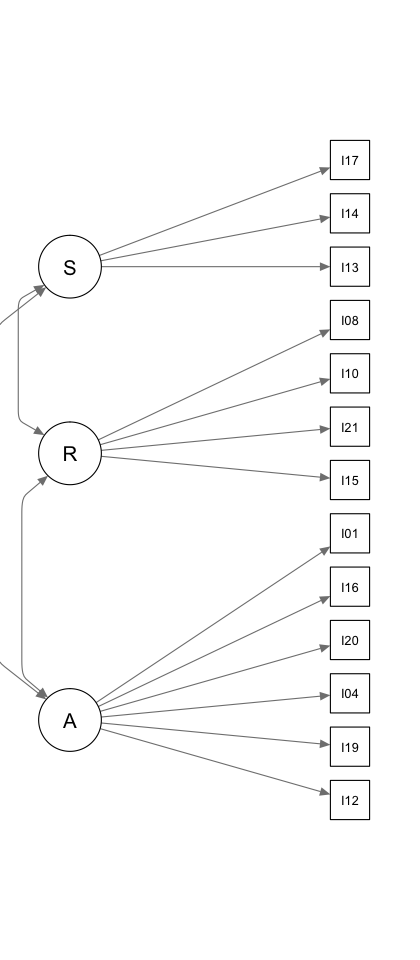
\includegraphics[width=0.25\textwidth]{images/appendix/imms-multidimensional-model.png} &
 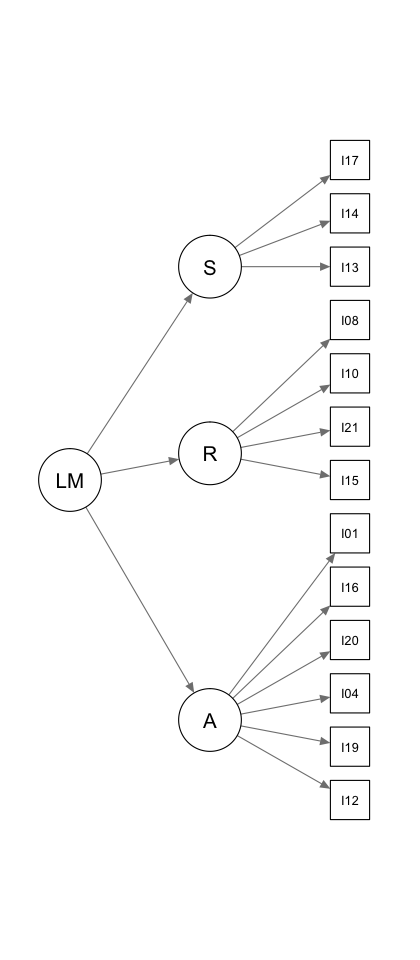
\includegraphics[width=0.25\textwidth]{images/appendix/imms-second-order-factor-model} &
 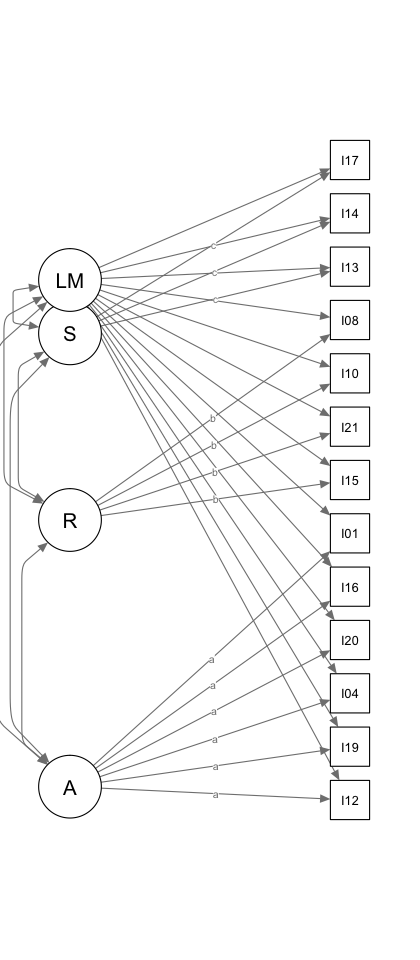
\includegraphics[width=0.25\textwidth]{images/appendix/imms-bi-factor-model.png} \\
 {\scriptsize multidimensional model} & {\scriptsize second-order factor model} & {\scriptsize bi-factor model} \\
 \end{tabular}
 \fautor
\end{figure}
\newpage

Instead to load in the scale of \emph{A: attention}, the Items 08, 10 and 21 loaded in the scale of \emph{R: Relevance}. The Item 08 - \aspas{\emph{A atividade foi muito abstrata que foi difícil manter minha atenção}} as an adapted and translated version of \aspas{The lesson was so abstract that it was hard to keep my attention on it} - was understood by the participants in the sense of abstraction rather than keeping attention, thereby this item has more concordance with the scale of \emph{R: Relevance}. The Item 10 - \aspas{O ambiente em que foi executada a atividade pareceu sem graça e desagradável} as an adapted and translated version of \aspas{The pages of this lesson looked dry and unappealing} - was understood in the sense of quality of the CL session rather than keeping focus, thereby this item lacks of concordance with the scale of \emph{A: Attention}. The Item 21 - \aspas{\emph{O ambiente e as tarefas da atividade foram chatos ou entediantes}} as an adapted and translated version of \aspas{The style of writing was boring} - was understood by the participants in the sense of quality rather than feeling bored, thereby this item is correlated with the scale of \emph{R: Relevance}. The Item 13 - \aspas{\emph{A atividade teve coisas que estimularam minha curiosidade}} as an adapted and translated version of \aspas{The lesson had things that stimulated my curiosity} - and the Item 17 - \aspas{\emph{Aprendi algumas coisas que foram surpreendentes e/ou inesperadas}} as an adapted version of \aspas{Aprendi algumas coisas que foram surpreendentes e/ou inesperadas} - were understood by the participants in the sense of feeling comfortable rather than playing close attention, thereby these both items loaded in the scale of \emph{S: Satisfaction} rather than loaded in the scale of \emph{A: attention}.

\autoref{tab:imms-goodness-fit} shows the goodness fit statistics for the models tested in the validation of the adapted Portuguese IMMS. The results presented in this table indicate that all the models have adequate goodness fit indices for all the samples (the global sample, and the samples obtained over the second and third empirical studies). Based on these results, the model that best fits the global sample is the bi-factor model with ${\chi}^2 = 22.29$ that outperforms the multidimensional model (${\chi}^2 = 26.39$), and the second-order factor model (${\chi}^2 = 26.39$). The AGFI index has the same value in the multidimensional and second-order model, and these indices are outperformed by the bi-factor model with $TLI = 0.99$ and $CFI = 0.97$. The RMSEA of all models indicates good fit with values less than 0.08.

%latex.default(round(fitMeasures_df, 2), caption = paste("Goodness of fit statistics",     in_title), size = "scriptsize", longtable = T, ctable = F,     landscape = F, rowlabel = "", where = "!htbp", file = filename,     append = T)%
\setlongtables{\footnotesize
\begin{longtable}{lrrrrrrrr}
\caption{Goodness of fit statistics in the validation of the adapted Portuguese IMMS}
\tabularnewline
\hline\hline
\multicolumn{1}{l}{}&\multicolumn{1}{c}{df}&\multicolumn{1}{c}{${\chi}^2$}&\multicolumn{1}{c}{AGFI}&\multicolumn{1}{c}{TLI}&\multicolumn{1}{c}{CFI}&\multicolumn{1}{c}{RMSEA}&\multicolumn{1}{c}{CI.lwr}&\multicolumn{1}{c}{CI.upr}\tabularnewline
\hline
\endfirsthead\caption[]{\em (continued)} \tabularnewline
\hline
\multicolumn{1}{l}{}&\multicolumn{1}{c}{df}&\multicolumn{1}{c}{${\chi}^2$}&\multicolumn{1}{c}{AGFI}&\multicolumn{1}{c}{TLI}&\multicolumn{1}{c}{CFI}&\multicolumn{1}{c}{RMSEA}&\multicolumn{1}{c}{CI.lwr}&\multicolumn{1}{c}{CI.upr}\tabularnewline
\hline
\endhead
\hline
\multicolumn{9}{r}{\tiny df: degree of freedom; AGFI: Adjusted Goodness of Fit Index; CFI: Comparative Fit Index; TLI: Tucker-Lewis Index;}\tabularnewline \multicolumn{9}{r}{\tiny RMSEA: Root Mean Square Error of Approximation}
\endfoot
\label{tab:imms-goodness-fit}
Global sample: Multidimensional model&$19.07$&$26.39$&$1.00$&$0.98$&$0.93$&$0.06$&$ 0$&$0.11$\tabularnewline
Global sample: Second-order factor model&$19.07$&$26.39$&$1.00$&$0.98$&$0.93$&$0.06$&$ 0$&$0.11$\tabularnewline
Global sample: Bi-factor model&$18.62$&$22.29$&$1.00$&$0.99$&$0.97$&$0.04$&$ 0$&$0.10$\tabularnewline \hline
Second study: Multidimensional model&$12.04$&$13.65$&$1.00$&$0.99$&$0.97$&$0.05$&$ 0$&$0.14$\tabularnewline
Second study: Second-order model&$12.04$&$13.65$&$1.00$&$0.99$&$0.97$&$0.05$&$ 0$&$0.14$\tabularnewline
Second study: Bi-factor model&$11.51$&$12.14$&$1.00$&$1.00$&$0.99$&$0.03$&$ 0$&$0.14$\tabularnewline \hline
Third study: Multidimensional model&$12.65$&$13.83$&$0.99$&$0.99$&$0.97$&$0.04$&$ 0$&$0.13$\tabularnewline
Third study: Second-order factor model&$12.65$&$13.83$&$0.99$&$0.99$&$0.97$&$0.04$&$ 0$&$0.13$\tabularnewline
Third study: Bi-factor model&$14.08$&$16.55$&$0.99$&$0.97$&$0.95$&$0.06$&$ 0$&$0.14$\tabularnewline
\hline
\end{longtable}
}

In relation to the data collected in each empirical study, the goodness of fit statistics (shown in \autoref{tab:imms-goodness-fit}) for the validation of the adapted Portuguese IMMS have slight differences. For the data collected over the second empirical study, the bi-factor model with ${\chi}^2=12.14$ fits better than the multidimensional model and the second-order factor model. For the data collected over the third empirical study, the multidimensional model and the second-order factor model with ${\chi}^2=13.83$ outperform the bi-factor model (${\chi}^2=16.555$), but there are not difference in the AGFI index. With the data collected over the third empirical study, the multidimensional model and second-order factor model with $TLI=0.99$ and $CFI=0.97$ outperform the bi-factor model ($TLI = 0.97$ and $CFI = 0.95$).

\autoref{tab:imms-factor-loading} shows the summary of the factor analysis conducted with the global sample for the adapted Portuguese IMMS. The factor loadings, eigenvalues, cumulative variance and proportion explained by the items indicates the emergence of tree factors: Attention (F1), Relevance (F2), and Satisfaction (F3). The items in the first factor (F1: Attention) have strong primary loadings with values greater than 0.6, and the majority of proportion (50\%) is explained by the first factor. These results are similars to the findings obtained in previous validation of the IMMS conducted by \citeonline{LoorbachPetersKarremanSteehouder2015, CookBeckmanThomasThompson2009, HuangHew2016}. According to the cut-off value defined by \citeonline{Yurdugul2008}, the first eigenvalue has a level of $3.9$ indicating stability in the Cronbach’s $\alpha$ for a sample size ($N=110$) between 100 to 300 observation .

%latex.default(fa_summary_df, caption = paste("Summary of exploratory and confirmatory factor analysis for the",     in_title), size = "small", longtable = T, ctable = F, landscape = F,     rowlabel = "", where = "!htbp", file = filename, append = T)%
\setlongtables{\footnotesize
\begin{longtable}{lrrr}\caption{Summary of factor analysis for the adapted Portuguese IMMS} \tabularnewline
\hline\hline
\multicolumn{1}{l}{}&\multicolumn{1}{c}{MR1}&\multicolumn{1}{c}{MR2}&\multicolumn{1}{c}{MR3}\tabularnewline
\hline
\endfirsthead\caption[]{\em (continued)} \tabularnewline
\hline
\multicolumn{1}{l}{}&\multicolumn{1}{c}{MR1}&\multicolumn{1}{c}{MR2}&\multicolumn{1}{c}{MR3}\tabularnewline
\hline
\endhead
\hline
\multicolumn{4}{r}{\tiny CFI: 0.966; TLI: 0.989; df: 18.619; $chi^2$: 22.291; p-value: 0.25; RMSEA: 0.043 [0, 0.104];}
\endfoot
\label{tab:imms-factor-loading}
\emph{A: Attention} & & & \tabularnewline
Item12: \emph{A forma como a informação foi organizada no ambiente ...}&$ 0.857$&$-0.198$&$ 0.203$\tabularnewline
Item19: \emph{O feedback ou outros elementos fornecidos na atividade, ...}&$ 0.785$&$-0.004$&$ 0.243$\tabularnewline
Item04: \emph{O ambiente e tarefas da atividade foram atraentes}&$ 0.738$&$-0.304$&$ 0.204$\tabularnewline
Item20: \emph{A variedade de tarefas e coisas no ambiente, ajudou a ...}&$ 0.726$&$-0.133$&$ 0.270$\tabularnewline
Item16: \emph{As tarefas e sua organização na atividade transmitiram a ...}&$ 0.693$&$-0.241$&$ 0.334$\tabularnewline
Item01: \emph{Houve algo interessante no início desta atividade que chamou ...}&$ 0.653$&$-0.337$&$ 0.234$\tabularnewline \hline
\emph{R: Relevance} & & & \tabularnewline
Item15: \emph{A quantidade de tarefas repetitivas na atividade na atividade me ...}&$-0.087$&$ 0.614$&$-0.125$\tabularnewline
Item21: \emph{O ambiente e as tarefas da atividade foram chatos ou entediantes}&$-0.321$&$ 0.662$&$-0.144$\tabularnewline
Item10: \emph{O ambiente em que foi executada a atividade pareceu sem graça ...}&$-0.347$&$ 0.625$&$-0.076$\tabularnewline
Item08: \emph{A atividade foi muito abstrata que foi difícil manter minha atenção}&$ 0.011$&$ 0.484$&$-0.179$\tabularnewline \hline
\emph{S: Satisfaction} & & & \tabularnewline
Item13: \emph{A atividade teve coisas que estimularam minha curiosidade}&$ 0.307$&$-0.360$&$ 0.810$\tabularnewline
Item14: \emph{Eu realmente gostei de participar na atividade}&$ 0.434$&$-0.343$&$ 0.644$\tabularnewline
Item17: \emph{Aprendi algumas coisas que foram surpreendentes e/ou inesperadas}&$ 0.388$&$-0.104$&$ 0.568$\tabularnewline \hline
SS loadings&$ 3.995$&$ 2.019$&$ 1.849$\tabularnewline
Cumulative Var&$ 0.307$&$ 0.463$&$ 0.605$\tabularnewline
Proportion Explained&$ 0.508$&$ 0.257$&$ 0.235$\tabularnewline
\hline
\end{longtable}
}

\subsection{Reliability Tests of the Adapted Portuguese IMMS}

The overall and internal consistency of the adapted Portuguese IMMS had been evaluated by reliability tests in the global sample, and in the data collected over each empirical study (the second and third empirical studies). \autoref{tab:reliability-IMMS} shows the results of the reliability tests in which the Cronbach's alpha ($\alpha$) for the Level of Motivation have good overall consistency ($\alpha=0.909$) for the global sample and the data collected in the second and third empirical studies with values greater than 0.80. The Cronbach's $\alpha$ in the scales of \emph{A: Attention}, \emph{R: Relevance}, \emph{S: Satisfaction} indicate good consistency and high reliability for all the samples with values greater than $0.70$ and $0.80$. The only exception had been found in the scale of \emph{R: Relevance} for the data collected over the third empirical study in which the Cronbach's $\alpha$ with value $0.66$ indicates questionable reliability, but this value is close to $0.70$, thereby the reliability is considered acceptable.

%latex.default(rel_summary_df, caption = paste("Result of reliability analysis for the",     in_title), size = "small", longtable = T, ctable = F, landscape = F,     rowlabel = "", where = "!htbp", file = filename, append = T)%
\setlongtables{\small
\begin{longtable}{lrrr}\caption{Result of reliability analysis for the adapted Portuguese IMMS} \tabularnewline
\hline\hline
\multicolumn{1}{l}{Cronbach's alpha ($\alpha$)}&\multicolumn{1}{c}{Global}&\multicolumn{1}{c}{Second Study}&\multicolumn{1}{c}{Third Study}\tabularnewline
\hline
\endfirsthead\caption[]{\em (continued)} \tabularnewline
\hline
\multicolumn{1}{l}{Cronbach's alpha ($\alpha$)}&\multicolumn{1}{c}{Global}&\multicolumn{1}{c}{Second Study}&\multicolumn{1}{c}{Third Study}\tabularnewline
\hline
\endhead
\hline
\endfoot
\label{tab:reliability-IMMS}
\emph{Level of Motivation}&$0.909$&$0.930$&$0.874$\tabularnewline
\emph{A: Attention}&$0.918$&$0.930$&$0.900$\tabularnewline
\emph{R: Relevance}&$0.728$&$0.748$&$0.696$\tabularnewline
\emph{S: Satisfaction}&$0.851$&$0.836$&$0.876$\tabularnewline
\hline
\end{longtable}}

Separate reliability tests had also been conducted in the adapted Portuguese IMMS for the collected data in each empirical study and by dividing this data into: responses from students who participated in non-gamified CL sessions (\emph{non-gamified}), responses from students who participated in ontology-based CL sessions (\emph{ont-gamified}), and responses from students who participated in CL sessions that had been gamified without using ontologies (\emph{w/o-gamified}). \autoref{tab:reliability-IMMS-samples} shows the results of these reliability tests, where the Cronbach's $\alpha$ in the majority of scales and groups indicate good ($\alpha$ in $0.80$s) and excellent ($\alpha$ in $0.90$s) internal consistency. The only questionable internal consistency occurs in the scale of \emph{R: Relevance} for the data collected over the third study in the \aspas{\emph{w/o-gamified}} group with a Cronbach's $\alpha$ of $0.684$, but this value is close to the threshold of 0.7 which by this internal consistency is considered as acceptable.

%latex.default(rel_summary_df, caption = paste("Result of reliability analysis for the",     in_title), size = "small", longtable = T, ctable = F, landscape = F,     rowlabel = "", where = "!htbp", file = filename, append = T)%
\setlongtables{\small
\begin{longtable}{lrrrr}\caption{Results of reliability tests in the adapted Portuguese IMMS for each empirical study} \tabularnewline
\hline\hline
\multicolumn{1}{l}{Cronbach's alpha ($\alpha$)}&\multicolumn{1}{c}{Global}&\multicolumn{1}{c}{\emph{non-gamified}}&\multicolumn{1}{c}{\emph{ont-gamified}}&\multicolumn{1}{c}{\emph{w/o-gamified}}\tabularnewline
\hline
\endfirsthead\caption[]{\em (continued)} \tabularnewline
\hline
\multicolumn{1}{l}{Cronbach's alpha ($\alpha$)}&\multicolumn{1}{c}{Global}&\multicolumn{1}{c}{\emph{non-gamified}}&\multicolumn{1}{c}{\emph{ont-gamified}}&\multicolumn{1}{c}{\emph{w/o-gamified}}\tabularnewline
\hline
\endhead
\hline
\endfoot
\label{tab:reliability-IMMS-samples} 
\emph{Second study}: Level of Motivation&$0.930$&$0.932$&$0.926$& \tabularnewline
\emph{Second study}: Attention&$0.930$&$0.935$&$0.915$& \tabularnewline
\emph{Second study}: Relevance&$0.748$&$0.728$&$0.784$& \tabularnewline
\emph{Second study}: Satisfaction&$0.836$&$0.851$&$0.817$& \tabularnewline \hline
\emph{Third study}: Level of Motivation&$0.874$& &$0.886$&$0.866$\tabularnewline
\emph{Third study}: Attention&$0.900$& &$0.924$&$0.881$\tabularnewline
\emph{Third study}: Relevance&$0.696$& &$0.725$&$0.684$\tabularnewline
\emph{Third study}: Satisfaction&$0.876$& &$0.884$&$0.889$\tabularnewline
\hline
\end{longtable}}




